\subsection{Беззнаковые числа}

\begin{frame}
	\tableofcontents[currentsection,currentsubsection]
\end{frame}

\begin{frame}[t]{Один байт}
	\begin{itemize}
		\item
			Любое целое число можно представить в двоичной системе счисления:
			\[ 150 = 128 + 16 + 4 + 2 = \t{1001~0110}_2 \]
		\item
			Есть младшие (менее значимые) знаки/биты, есть старшие.
		\item
			На ближайших слайдах работает внутри 1 байта (8 бит).
		\item
			Пока все промежуточные результаты вычислений от $0$ до $255$, нет никаких проблем "--- считаем и считаем.
	\end{itemize}
	Что делать, если произошло переполнение (overflow/underflow)?
	Результат точно не сохраним.
	\begin{enumerate}
		\item Можно вызвать ошибку.
		\item Можно откинуть младшие знаки.
		\item Можно откинуть старшие знаки.
	\end{enumerate}
	Если откинем младшие, то $254+1-1\neq 254$, что неудобно, если мы хотим точные вычисления.
\end{frame}

\begin{frame}
	\begin{center}
		
\includegraphics[scale=0.3]{will-i-use-algebra.jpg}
	\end{center}
\end{frame}

\begin{frame}
	А вот если считаем, что откидываем старшие, то получаем коммутативное кольцо с единицей $\mathbb{Z}/256\mathbb{Z}$.

	\begin{center}
		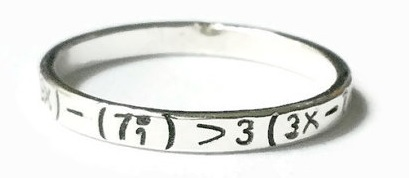
\includegraphics[scale=0.5]{math-ring.jpg}
	\end{center}

	\begin{itemize}
		\item
			По сути "--- просто арифметика, где все числа берутся по модулю 256.
		\item
			Сложение, вычитание, умножение в таких объектах прекрасно определены и непротиворечивы.
		\item
			Можно делать что угодно, и мы всегда получим корректный результат по модулю 256.
		\item
			В железе реализовать просто "--- считаем только последние 8 бит результата.
	\end{itemize}
\end{frame}

\begin{frame}{Деление}
	С делением хуже (деление "--- обратное к умножению).

	После взятия по модулю иногда можно однозначно восстановить ответ, а иногда нет (на алгебре расскажут, когда):
	\begin{align*}
	    34 / 17 &= 2 \\
		4386 / 17 &= 258 = 2 \mod 256 \\
		48 / 4 &= 12 \\
		\underbrace{(256+48)}_{304} / 4 &= 76
	\end{align*}
	Поэтому деление всегда считает, что у нас числа помещаются в 8 бит, и делим мы с остатком.
\end{frame}
